\subsection*{Задание 1.4}


\underline{Условие:} Все потоки случайных событий считать пуассоновскими. Если все операторы заняты, звонок теряется. Рассмотреть систему без ограничений на длину очереди, учитывающей фактор ухода клиентов из очереди (среднее приемлемое время ожидания – Tw секунд). Построить график средней длины очереди в зависимости от числа операторов (вплоть до числа каналов, соответствующего 1$\%$  отказов в системе без очереди). Построить график, иллюстрирующий коэффициент загрузки операторов. Построить график математического ожидания времени пребывания клиентов в очереди.\par

\underline{Решение:}\par

Для расчета вероятности, при которой операторы не будут заняты, можно воспользоваться формулой 15:\par

\begin{equation}
     P_{0}=\frac{1}{ \sum _{i=0}^{N}\frac{ \lambda ^{i}}{i! \cdot  \mu ^{i}}+\frac{ \lambda ^{N}}{N! \cdot  \mu ^{N}} \cdot  \sum _{k=1}^{\infty}\frac{ \lambda ^{k}}{ \prod_{j=1}^{k} \left( N \cdot  \mu +j \cdot  \upsilon  \right) }}  
\end{equation} \par

где  \(  \upsilon -  \) интенсивность выхода из очереди.\par

Для расчета математического ожидания длины очереди можно воспользуемся формулой:

\begin{equation}
    \overline{Q}= \sum _{k=1}^{\infty}\frac{k \cdot  \lambda ^{k}}{ \prod_{j=1}^{k} \left( N \cdot  \mu +j \cdot  \upsilon  \right) } \cdot \frac{ \lambda ^{N}}{N! \cdot  \mu ^{N}} \cdot P_{0}
\end{equation} \par

Для расчета среднего количества занятых операторов можно воспользуемся формулой:

 \begin{multline} 
    \overline{N} = \\ P_{0}  \cdot  \left(  \sum _{i=1}^{N}\frac{ \lambda ^{i}}{ \left( i-1 \right) ! \cdot  \mu ^{i}}+ \frac{ \lambda ^{N}}{ \left( N-1 \right) ! \cdot  \mu ^{N}} \cdot   \sum _{k=1}^{\infty}\frac{ \lambda ^{k}}{ \prod_{j=1}^{k} \left( N \cdot  \mu +j \cdot  \upsilon  \right) } \right) 
\end{multline} \par

\begin{figure}[H]
	\begin{center}
        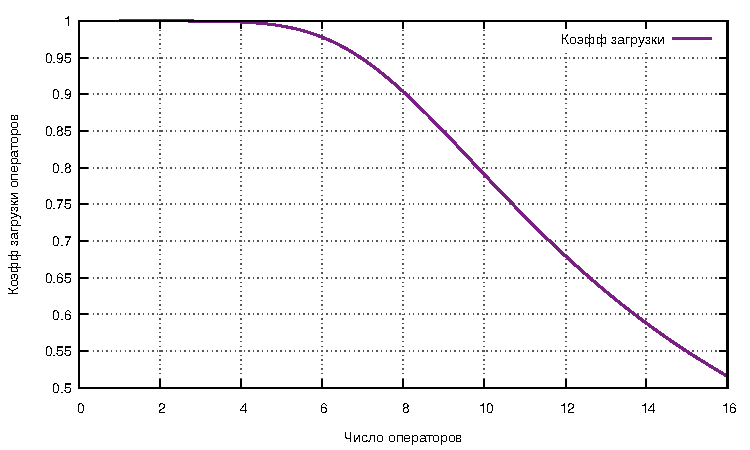
\includegraphics{/z1.4/ninftime.pdf}
        \caption{Зависимость коэффициента загрузки операторов от их общего количества}
	\end{center}
\end{figure}


\begin{figure}[H]
	\begin{center}
        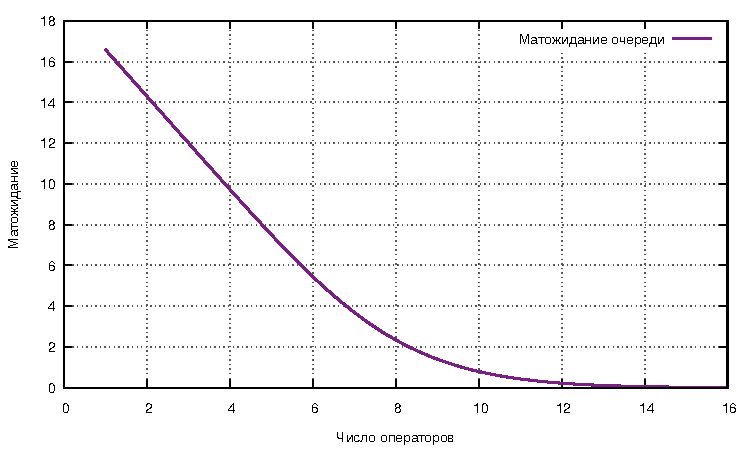
\includegraphics{/z1.4/qinftime.pdf}
        \caption{Зависимость математического ожидания длины очереди от количества операторов}
	\end{center}
\end{figure}


\begin{figure}[H]
	\begin{center}
        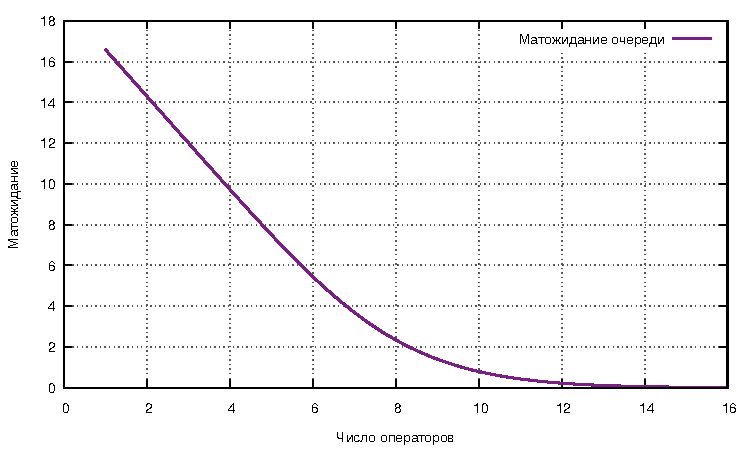
\includegraphics{/z1.4/qinftime.pdf}
        \caption{Зависимость математического ожидания времени ожидания в очереди от количества операторов}
	\end{center}
\end{figure}